\chapter{Il Protocollo}
\label{chap:protocollo}

In questo capitolo verrà trattato il protocollo proposto per l'implementazione
della Time-Lock Encryption sui DLT. Nella prima parte cercheremo di spiegare
l'idea che sta alla base, anche con l'ausilio di un esempio. Nella seconda parte
invece passeremo ad analizzare gli aspetti più formali, come le caratteristiche
dello Smart Contract che
serve implementare e i requisiti del DLT sui cui operare.

\section{L'idea}
\subsection{Versione base}
\label{subsec:versione-base}
Immaginiamo che Carol abbia bisogno di Time-Lock Encryption su un certo messaggio $ x $.
Per farlo decide farsi aiutare da Alice. Quest'ultima
impegna a conservare il messaggio e ha renderlo pubblico solo dopo un
certo istante di tempo $ \tau $.
Alice però vuole essere retribuita per la conservazione di $ x $. Viene quindi fissata
una ricompensa \textit{prize}.

Alice vuole essere sicura di
ottenere la ricompensa se rispetta il suo impegno. Allo stesso tempo Carol
vuole avere la certezza che Alice possa riscattare il premio solo se si comporta
in maniera corretta.
Carol inoltre non vuole che soggetti terzi partecipino all'accordo, perché desidera
che sia $ x $ sia l'accordo stesso rimangano segreti.
Per farlo decidono di usare uno smart contract.

\paragraph{Inizializzazione}
Nella fase iniziale Carol invia ad Alice il messaggio $ x $. Allo stesso tempo invia
allo smart contract una certa cifra in criptomoneta
che corrispone alla somma tra il premio \textit{prize} da corrispondere ad Alice e un
\textit{pawn} che le verrà ritornato al termine delle operazioni, un hash
crittografico del segreto $ x $, l'istante di tempo $ \tau $ e una tolleranza $ \delta $.
\begin{figure}[H]
	\centering
	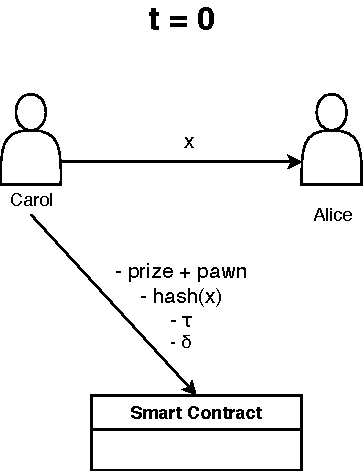
\includegraphics[width=0.3\linewidth]{images/chap_protocollo/base-creazione.pdf}
	\caption{Step 0}
\end{figure}


\paragraph{Pubblicazione}
Alice si impegna quindi a conservare il segreto, e lo rende noto al tempo $ t^{*} $
(con $ \tau \leq t^{*} \leq \tau + \delta $).\footnote{Il $ \delta $ serve a far si che
	Alice pubblichi puntualmente il messaggio. Se non ci fosse questo vincolo temporale
	potrebbe rilasciare il messaggio anche con molto ritardo rispetto a
	$ \tau $ ed ottenere comunque
	la ricompensa.}
Per farlo invia allo smart contract $ x $, ed in cambio ottiene il suo premio
\textit{price}.
Allo stesso tempo, Alice riottiene il \textit{pawn} che aveva versato in precedenza.
\footnote{Ad una prima analisi può sembrare che il \textit{pawn} sia inutile,
	ma in realtà è necessario per proteggersi da alcuni tipi di attacchi.
	Le ragioni dettagliate verranno discusse nei capitoli successivi.}
\begin{figure}[H]
	\centering
	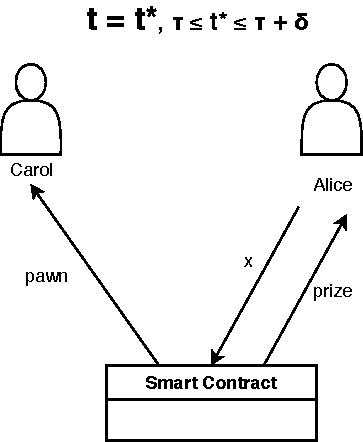
\includegraphics[width=0.3\linewidth]{images/chap_protocollo/base-pubblicazione.pdf}
	\caption{Step ok}
\end{figure}

\paragraph{Accesso al messaggio}
Dopo il tempo $ t^{*} $, ossia dopo che Alice ha inviato $ x $ allo smart contract,
il messaggio diventa pubblico e
chiunque può leggerlo.
\begin{figure}[H]
	\centering
	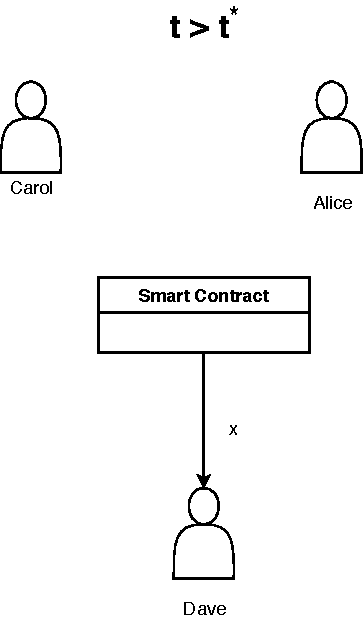
\includegraphics[width=0.3\linewidth]{images/chap_protocollo/base-leggi.pdf}
	\caption{Step leggi}
\end{figure}

\paragraph{Pubblicazione anticipata}
Cosa succede se Alice prova a riscattare il premio prima dell'istante $ \tau $?
Semplicemente lo smart contract rifiuta la sua richiesta.
\begin{figure}[H]
	\centering
	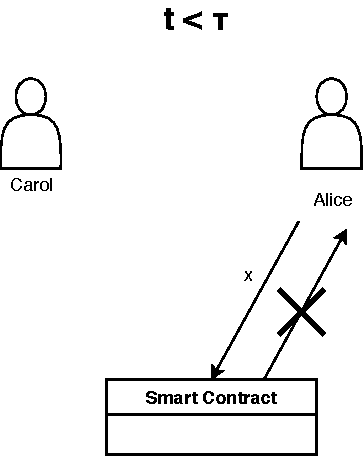
\includegraphics[width=0.3\linewidth]{images/chap_protocollo/base-anticipo.pdf}
	\caption{Step anticipo}
\end{figure}

\paragraph{Leak}
E se Alice cede (volontariamente o a causa di un furto)
il segreto ad Eve prima del tempo $ \tau $?
In questo caso Eve può usare $ x $ per ottenere una ricompensa
\textit{counterprize} \footnote{dove \textit{counterprize} $ \ll $ \textit{prize}.
	Le ragioni di questo vincolo sono spiegate al capitolo [...]}
Il riscatto del \textit{counterprize} impedisce ad Alice di ottenere il suo premio.
È evidente che l'interesse di Alice è quello di mantenere $ x $ segreto.
\begin{figure}[H]
	\begin{minipage}{0.5\textwidth}
		\centering
		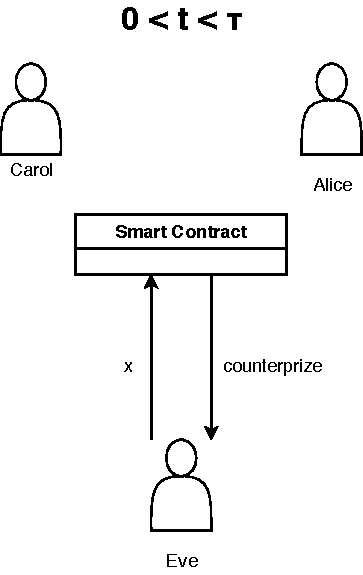
\includegraphics[width=.7\linewidth]{images/chap_protocollo/base-leak-1.pdf}
		\caption{Leak 1}
	\end{minipage}\hfill
	\begin{minipage}{0.5\textwidth}
		\centering
		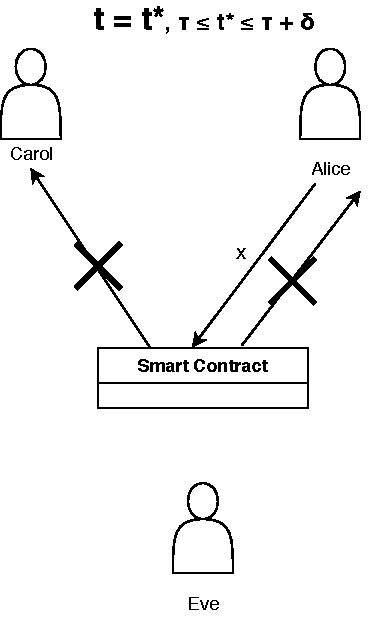
\includegraphics[width=.7\linewidth]{images/chap_protocollo/base-leak-2.pdf}
		\caption{Leak 2}
	\end{minipage}
\end{figure}


\subsection{Versione avanzata}
Facciamo notare che nella versione base (\ref{subsec:versione-base})
Alice conosce sin
dall'inizio il messaggio
$ x $, perché le è stato affidato nella prima fase del processo.
Ma se Carol volesse che il messaggio rimanga segreto anche ad Alice?
Per soddisfare questa condizione Alice ha bisogno di (almeno) un altro collaboratore,
Bob, e di un
algoritmo di \textbf{secret sharing}. \footnote{Un algoritmo di secret sharing
	è un algoritmo che permette di
	distribuire un certo segreto tra un gruppo di partecipanti, ad ognuno dei quali viene
	assegnato uno \textit{share}. Il segreto può essere ricostruito solo unendo un certo
	numero di share.}

\paragraph{Inizializzazione}
Alice, utilizzando un algoritmo di secret sharing, ottiene due \textit{share}
$ x_A $ e $ x_B $. Invia questi share rispettivamente ad Alice e a Bob, ed inizializza
lo smart contract versando due prize e due pawn, inviando gli hash crittografici
degli share, il tempo $ \tau $ e la tolleranza $ \delta $.
\begin{figure}[H]
	\centering
	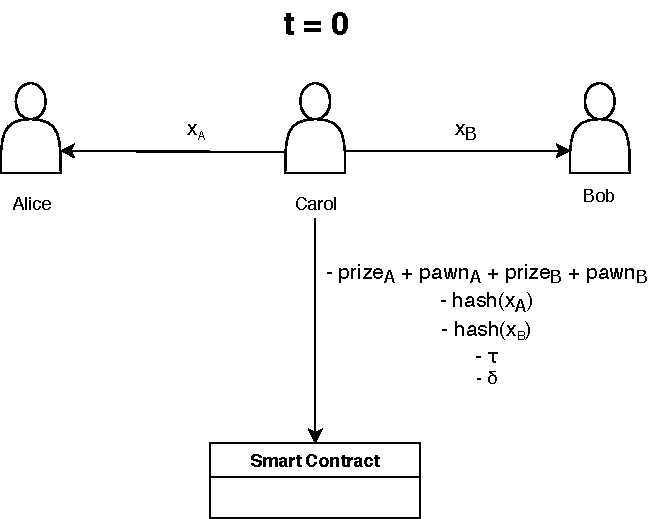
\includegraphics[width=0.6\linewidth]{images/chap_protocollo/avanzato-creazione.pdf}
	\caption{Avanzato - Inizializzazione}
\end{figure}



\paragraph{Pubblicazione}
Alice e Bob pubblicano i loro share rispettivamente al tempo $ t^*_A $ e $ t^*_B $
(con $ \tau \leq t^*_A \leq \tau + \delta $, $ \tau \leq t^*_B \leq \tau + \delta $).
In cambio ottengono il loro
\textit{price},
ed allo stesso tempo Alice riottiene i rispettivi \textit{pawn} che aveva versato
in precedenza.
\begin{figure}[H]
	\begin{minipage}{0.5\textwidth}
		\centering
		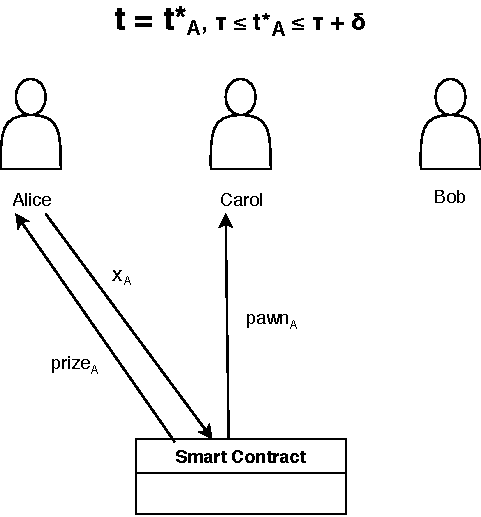
\includegraphics[width=.7\linewidth]{images/chap_protocollo/avanzato-pubblicazione-a.pdf}
		\caption{Leak 1}
	\end{minipage}\hfill
	\begin{minipage}{0.5\textwidth}
		\centering
		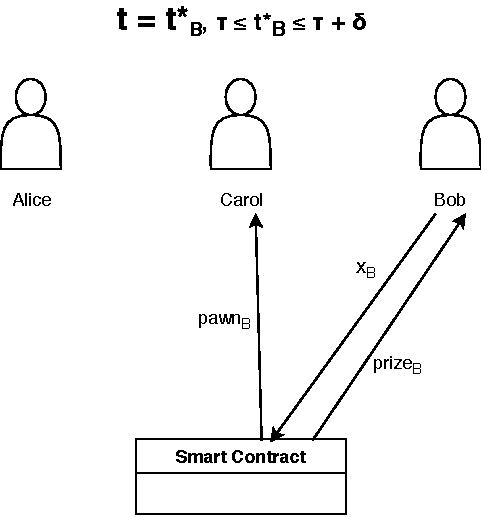
\includegraphics[width=.7\linewidth]{images/chap_protocollo/avanzato-pubblicazione-b.pdf}
		\caption{Leak 2}
	\end{minipage}
\end{figure}

\paragraph{Accesso al messaggio}
Dopo il tempo $ t^* = max(t^*_A, t^*_B) $, ossia dopo che sia Alice sia Bob
hanno inviato $ x_A $ ed $ x_B $
allo smart contract, chiunque può leggere gli share dallo smart contract e quindi
ricostruire il messaggio $ x $.
\begin{figure}[H]
	\centering
	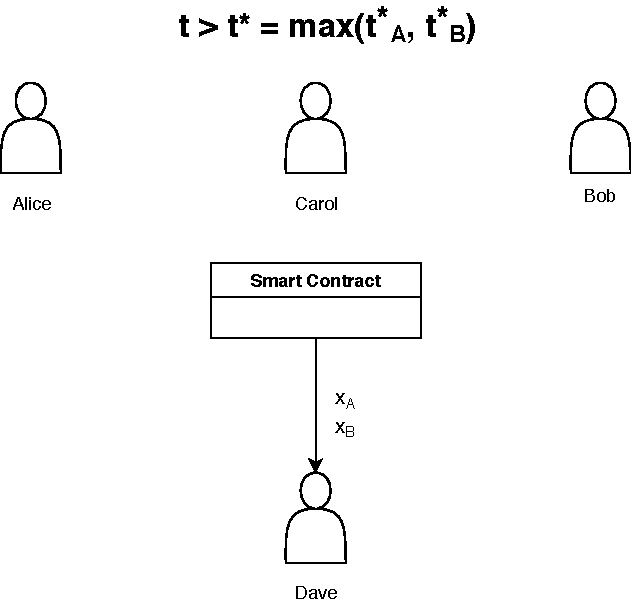
\includegraphics[width=0.5\linewidth]{images/chap_protocollo/avanzato-leggi.pdf}
	\caption{Step leggi}
\end{figure}

\paragraph{Leak}
Cosa succede se Bob cede il suo share ad Eve prima del tempo $ \tau $?
In questo caso Eve può usare $ x_B $ per ottenere una ricompensa
\textit{counterprize}
Il riscatto del \textit{counterprize} impedirebbe a Bob di ottenere il suo premio.
Da notare che se Alice si comporta in maniera corretta, ossia se tiene segreto il
suo share, è in grado di ottenere la sua ricompensa indipendentemente dal comportamento
di Bob.
\begin{figure}[H]
	\centering
	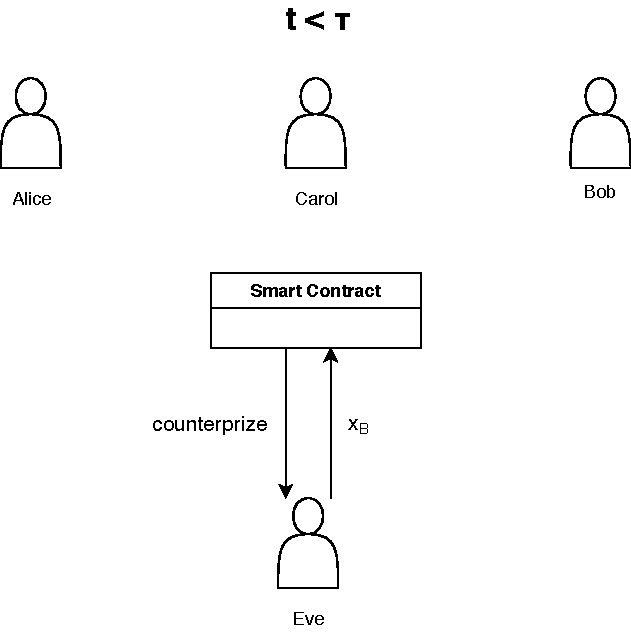
\includegraphics[width=0.4\linewidth]{images/chap_protocollo/avanzato-leak-1.pdf}
	\caption{Step leggi}
\end{figure}

\begin{figure}[H]
	\begin{minipage}{0.5\textwidth}
		\centering
		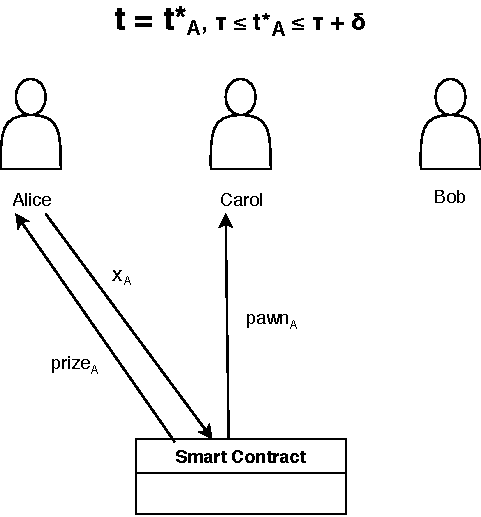
\includegraphics[width=.8\linewidth]{images/chap_protocollo/avanzato-leak-2-a.pdf}
		\caption{Leak 1}
	\end{minipage}\hfill
	\begin{minipage}{0.5\textwidth}
		\centering
		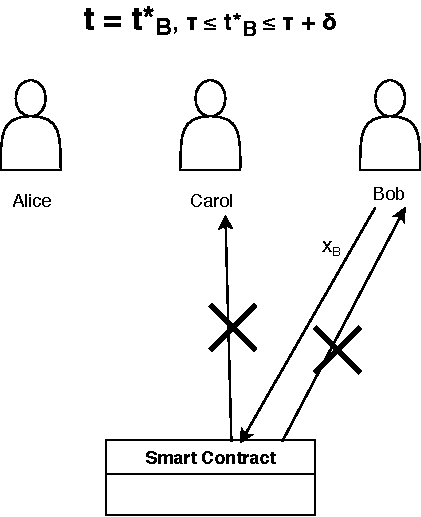
\includegraphics[width=.71\linewidth]{images/chap_protocollo/avanzato-leak-2-b.pdf}
		\caption{Leak 2}
	\end{minipage}
\end{figure}

Abbiamo visto un esempio con la partecipazione di tre soggetti, ma il protocollo
può essere analogamente implementato con $ N $ partecipanti, dove $ N \geq 3 $.

